\documentclass[runningheads,a4paper]{llncs}

\usepackage[american]{babel}

\usepackage{graphicx}

%extended enumerate, such as \begin{compactenum}
\usepackage{paralist}

%put figures inside a text
%\usepackage{picins}
%use
%\piccaptioninside
%\piccaption{...}
%\parpic[r]{\includegraphics ...}
%Text...

%Sorts the citations in the brackets 
%\usepackage{cite}

%for easy quotations: \enquote{text}
\usepackage{csquotes}

\usepackage[T1]{fontenc}

%enable margin kerning
\usepackage{microtype}

%better font, similar to the default springer font
\usepackage[%
rm={oldstyle=false,proportional=true},%
sf={oldstyle=false,proportional=true},%
tt={oldstyle=false,proportional=true,variable=true},%
qt=false%
]{cfr-lm}
%
%if more space is needed, exchange cfr-lm by mathptmx
%\usepackage{mathptmx}

%for demonstration purposes only
\usepackage[math]{blindtext}

\usepackage[
%pdfauthor={},
%pdfsubject={},
%pdftitle={},
%pdfkeywords={},
bookmarks=false,
breaklinks=true,
colorlinks=true,
linkcolor=black,
citecolor=black,
urlcolor=black,
%pdfstartpage=19,
pdfpagelayout=SinglePage
]{hyperref}
%enables correct jumping to figures when referencing
\usepackage[all]{hypcap}

\usepackage[capitalise,nameinlink]{cleveref}
%Nice formats for \cref
\crefname{section}{Sect.}{Sect.}
\Crefname{section}{Section}{Sections}
\crefname{figure}{Fig.}{Fig.}
\Crefname{figure}{Figure}{Figures}

\usepackage{xspace}
%\newcommand{\eg}{e.\,g.\xspace}
%\newcommand{\ie}{i.\,e.\xspace}
\newcommand{\eg}{e.\,g.,\ }
\newcommand{\ie}{i.\,e.,\ }

%introduce \powerset - hint by http://matheplanet.com/matheplanet/nuke/html/viewtopic.php?topic=136492&post_id=997377
\DeclareFontFamily{U}{MnSymbolC}{}
\DeclareSymbolFont{MnSyC}{U}{MnSymbolC}{m}{n}
\DeclareFontShape{U}{MnSymbolC}{m}{n}{
    <-6>  MnSymbolC5
   <6-7>  MnSymbolC6
   <7-8>  MnSymbolC7
   <8-9>  MnSymbolC8
   <9-10> MnSymbolC9
  <10-12> MnSymbolC10
  <12->   MnSymbolC12%
}{}
\DeclareMathSymbol{\powerset}{\mathord}{MnSyC}{180}

% correct bad hyphenation here
\hyphenation{op-tical net-works semi-conduc-tor}

\begin{document}

%Works on MiKTeX only
%hint by http://goemonx.blogspot.de/2012/01/pdflatex-ligaturen-und-copynpaste.html
%also http://tex.stackexchange.com/questions/4397/make-ligatures-in-linux-libertine-copyable-and-searchable
%This allows a copy'n'paste of the text from the paper
%\input glyphtounicode.tex
\pdfgentounicode=1

\title{KBID: Kerberos Bracelet Identification (Short Paper)}
%If Title is too long, use \titlerunning
%\titlerunning{Short Title}

%Single insitute
%\author{Joseph Carrigan \and Paul Martin \and Michael Rushanan}
%If there are too many authors, use \authorrunning
%\authorrunning{First Author et al.}
%\institute{Johns Hopkins University \{joseph.carrigan,pmartin,mrushan1\}@jhu.edu}

%Multiple insitutes
%Currently disabled
%
\iffalse
%Multiple institutes are typeset as follows:
\author{Firstname Lastname\inst{1} \and Firstname Lastname\inst{2} }
%If there are too many authors, use \authorrunning
%\authorrunning{First Author et al.}

\institute{
Insitute 1\\
\email{...}\and
Insitute 2\\
\email{...}
}
\fi
			
\maketitle

\begin{abstract}
The most common method for a user to gain access to a system, service, or resource is to provide a secret, often a password, that verifies her identity and thus authenticates her. Password-based authentication is considered strong only when the password meets certain length and complexity requirements, or when it is combined with other methods in multi-factor authentication. Unfortunately, many authentication systems do not enforce strong passwords due to a number of limitations; for example, the time taken to enter complex passwords. We present an authentication system that addresses these limitations by prompting a user for credentials once and then storing an authentication ticket in a wearable device that we call \textit{Kerberos Bracelet Identification} (KBID).  
\end{abstract}

\keywords{authentication, kerberos, wearables, passwords}

%%%%%%%%%%%%%%%%%%%%%%%%%%%%%%%%%%%%%%%%%%%%%%%%%%%%%%%%%%%%%%%%%%%%%%%%%%%%%%%
\section{Introduction}\label{sec:intro}
%%%%%%%%%%%%%%%%%%%%%%%%%%%%%%%%%%%%%%%%%%%%%%%%%%%%%%%%%%%%%%%%%%%%%%%%%%%%%%%
The use of modern computer systems almost always requires that a user prove their identity through some process of authentication.  Specifically, a user can authenticate using methods such as public key authentication, biometrics, and passwords; something you have, are, or know, respectively.  Password-based authentication remains the most widely used option for authentication because of its ease of use and simple design. %TODO: Citation here?

%this is the original of the paragraph below
%However, passwords have a human factor weakness.  Users often choose passwords that are too simplistic and easily guessed.  Thus, administrators encourage or force users to select more complex and longer passwords.  More complex and longer passwords decrease user satisfaction because entering the passwords is perceived as difficult.  This difficulty is compounded when the user enters a password incorrectly and has to re-enter it.  Additionally, the likelihood of entering a password incorrectly only increases with password complexity and length as does the time to enter and re-enter it.  The difficulty of entering a complex password rises to an unacceptable level very quickly in a medical or clinical setting, particularly when patient needs are urgent.  

However, passwords have a human factor weakness as users often choose passwords that are too simplistic and easily guessed~\cite{Yan:2004:PMS:1024867.1025014}.  Administrators and systems require users to select more complex passwords as a consequence; thus, decreasing user satisfaction as password selection becomes seemingly difficult. Worst yet, complex passwords interfere in critical workflow such as clinical care where a patient's need is most urgent.  

In this paper we describe an authentication system that requires the user to enter a password as infrequently as once a day.  Specifically, authentication information is stored on a wearable device, a bracelet in our case, and is transmitted to devices to which the user wishes to authenticate. The transmission between the bracelet and device is achieved via using the user's body as a communication medium~\cite{Barth:2008:BCB:1460257.1460273,chang:healthtech:2013}. Our goal is to reduce the impact on user satisfaction and workflow by removing most of the difficulty of using a complex password. 

While we focus on authentication in the medical community use case, we anticipate that other areas such as the financial sector may benefit from our system. In addition, it is important to note that this system is not a two-factor authentication solution. The bracelet is not a biometric component and does not provide any additional information outside of what it stores. It is meant to enhance the user experience and encourage the use of complex passwords. Finally, KBID is a work in progress.

%Our goal is to authenticate a user in less than one second provided that user has provided valid credentials once.   The hope is to reduce the resistance to strong password requirements by removing the vast majority events where the user is asked to enter a password.  %To put it simply, users will be more willing to use a strong password if they only have to enter it once a day as opposed to being prompted to enter the password each time they use a computer system.

%While we have focused on developing an authentication system for the medical community, there is nothing in the authentication system that prevents it from being used in other areas.  We anticipate that the financial sector may find our system interesting.

%It is important to note what this system is not.  This system is not a two factor authentication solution.  The bracelet should not be confused as the provider of additional authentication information outside of what it is instructed to hold.  There is no biometric component to this system.  This system is not a complete authentication system.  It is meant to be an enhancement to the user experience and to encourage the use of strong passwords by eliminating the need to repeatedly entering them. Finally, KBID is a work in progress.



%To use the system, the user will don a wearable device.  Currently we envision this device as a bracelet.  The user will approach a host computer equipped with a special hardware to communicate with the bracelet.  We will refer to this hardware as an authentication module.  The user will touch a sensor on the authentication module and the authentication module will communicate over the user's skin and determine that the user is not authenticated.  The authentication module will then communicate with a software client on the host computer and the software will prompt the user to log in.  The user will provide a username and password that will be validated with the back end authentication server.  If the user's credentials are valid, the server will provide authentication information to the client.  The client will instruct the user to touch the sensor on the authentication module again.  When the user touches the authentication module the client will send the authentication information to the authentication module which will in turn pass it over the user's skin to the bracelet where it will be stored.

%The next time the user wishes to authenticate to a host computer equipped with this system, the user will touch the authentication module.  The authentication module will ask the bracelet for the authentication information and the bracelet will provide it.  The authentication module will then send the authentication information to the client on the host computer.  The client will verify the validity of the authentication information with the authentication server.  If the authentication information is valid the client will unlock the host computer.  It is these subsequent authentication events that should take less than one second.

%If the user removes the bracelet, the bracelet has a means of detecting its removal.  When it detects its removal the bracelet will delete the authentication information it contains.  In order to continue using the system, the user must put the bracelet back on and re-authenticate using a username and a password.

%It is conceivable that users of computer systems in a clinical setting may not be able to use a keyboard and mouse due to sanitation concerns.  An additional benefit of this system is that clinicians could authenticate by making contact between the sensor and another part of their arm, such as the elbow, without compromising the sanitization of their hands.

%While we have focused on developing an authentication system for the medical community, there is nothing in the authentication system that prevents it from being used in other areas.  We anticipate that the financial sector may find our system interesting.

%At their developer conference in August 2015, Intel announced a wearable authentication solution.  The Intel solution has a very similar workflow and seems to achieve similar results.  However the Intel solution uses Bluetooth Low Energy (BLE).  We speculate that the Intel solution may be vulnerable to a range extending attack.  In the speculative attack, an attacker intercepts the BLE signal from the user's wearable device and the computer to which they are authenticated.  The attacker then rebroadcasts the BLE traffic over a longer distance, possibly by translating the traffic to another section of the RF spectrum during the retransmission process.  No authentication or paring is required since all the attacker is doing is receiving and then rebroadcasting BLE traffic from previously paired and authenticated equipment.  Our system reduces or eliminates this type of attack by requiring that the user be in physical contact with the authentication device to transmit authentication information.

%this is the original of the paragraph below
%It is important to note what this system is not.  This system is not a two factor authentication solution.  It is conceivable that this system could include a two factor authentication component but the bracelet should not be confused as the provider of additional authentication information outside of what it is instructed to hold.  There is no biometric component to this system.  Neither the bracelet nor the authentication module measure or store any information about the user's physical state.  In this system the user's body is simply the medium across which the authentication information is communicated.  This system is not a complete authentication system.  It is meant to be an enhancement to the user experience and to encourage the use of strong passwords by eliminating the need to repeatedly entering them.  As such there will be no discussion in the paper about access control, password hashing, and much of the intricacies of the of the authentication process.  For this research Kerberos was used as the authentication provider but it is important to note that this system will support the use of any authentication provider that requires the use of stored tokens or tickets.  It could also be enhanced to provide its own tokens or tickets, though that is beyond the scope of the planned research on this project.  Finally, KBID is a work in progress.

%%%%%%%%%%%%%%%%%%%%%%%%%%%%%%%%%%%%%%%%%%%%%%%%%%%%%%%%%%%%%%%%%%%%%%%%%%%%%%%
\section{Background}\label{sec:background}
%%%%%%%%%%%%%%%%%%%%%%%%%%%%%%%%%%%%%%%%%%%%%%%%%%%%%%%%%%%%%%%%%%%%%%%%%%%%%%%
KBID originates from the idea of integrating a wearable device to achieve some additional property in an authentication system (e.g., de-authentication). In particular, we are inspired by the design of zero-effort bilateral recurring authentication (ZEBRA) by Mare et al.~\cite{mare:zebra:2014}. In ZEBRA, a user wears a bracelet that encapsulates a wireless radio, accelerometer, and gyroscope; these components record and transmit wrist movements to a computer system that is currently being used. The computer system continually compares received movement measurements to input it receives from it's keyboard and mouse. If these two measurements are not correlated, the current session is de-authenticated. 

At the time, ZEBRA was only envisioned as a method to de-authenticate a user from a computer system and did not include a way to initially authenticate the user to the system.  Assuming that the user has already accepted wearing a device that will effectively de-authenticate them, adding functionality to rapidly authenticate them only increases the usefulness of the system.

We avoided using radio frequency (RF) emissions for two reasons.  First, RF by it's nature emits information into the environment.  That information, once emitted, can be received by various means.  Second, RF relies on the underlying communication being secure.  If a security flaw is discovered in an RF communication framework, e.g. Bluetooth low energy (BLE)~\cite{BLEATTACK}, then the systems as it exists could be vulnerable to the flaw.  Specifically, there is no need to alter or even monitor the information that is exchanged between the computer system and a wearable device.  An attacker would only need to extend the range of the wireless communication in order to gain access to the computer system.

% TODO: Unless we can be explicit about the human factor issues, I'd say drop this.
%We considered adding contacts to the wearable device.  This would allow the direct exchange of information over a closed circuit without the ability to use and extended range attack.  However, the human factors issues became clear when we considered the design.  Thus we were left with BCC.

We instead use body-coupled communication (BCC), or transmission of information over the human body as a medium. We are not the first to use BCC to transmit a secret. For example, Chang et al. introduce a system for key exchange over a body area network~\cite{chang:healthtech:2013}. By applying a very small voltage to the tissue of a dead mouse, they were able to communicate at a rate of 5Hz or 5 bits per second.  However, this data rate is not acceptable for our work as we would need to communicate authentication data of at least 256 bits, and this would take nearly a minute to transmit.  

%this is the original of the paragraph below
%We also wanted to be sure that the authentication information was non-transferable once the bracelet was holding it.  Thus we incorporated a feature in the design that would clear out the authentication information once it detected that the bracelet was removed.

We designed our authenticated bracelet to be non-transferrable (i.e., authenticating and then giving the bracelet to someone else). To support this feature, we zero all authentication information upon bracelet removal. 

%We also wanted to be sure that an authenticated bracelet was not transferable.  We incorporated a feature in the design that would clear out the authentication information once the bracelet was removed.

%Finally we wanted to provide an authentication model that was useful as a real world example.  Thus we incorporated a Kerberos server as the source of authentication.

%%%%%%%%%%%%%%%%%%%%%%%%%%%%%%%%%%%%%%%%%%%%%%%%%%%%%%%%%%%%%%%%%%%%%%%%%%%%%%%
\section{Related Work}\label{sec:related}
%%%%%%%%%%%%%%%%%%%%%%%%%%%%%%%%%%%%%%%%%%%%%%%%%%%%%%%%%%%%%%%%%%%%%%%%%%%%%%%

In addition to the ZEBRA, which we have described previously, there have been several previous attempts at developing wearable-authentication technology.  Two of note include the Bionym Nymi \cite{goode2014bring} and the Intel Authentication Bracelet \cite{idf2015intel}.  The Bionym Nymi is an authentication wristband that broadcasts a digitally signed authentication signal derived from a user's heartbeat to nearby devices using BLE~\cite{BLEoverview}.  The Intel Authentication Bracelet requires a user to log in to a system with a standard password.  A credential is then transmitted to the bracelet using BLE.  This credential is then broadcast to nearby bracelet-enabled devices in order to allow password-less login.

\subsubsection{Limitations of Existing Work}
Existing authentication wearables use wireless communication technology (typically BLE) to broadcast their authentication credentials.  Thus the devices are likely vulnerable to ghost-and-leech attacks \cite{czeskis2008rfids}.  Ghost-and-leech attacks occur when an attacker uses a more powerful radio transmitter than the transmitter found on a wireless device in order to capture and rebroadcast the wireless signal in order to fool a target into believing that the wireless device is in closer proximity to the target than it actually is.

%Related work can be divided into two key areas: authentication and deauthentication.  Authentication-based research looks at using wristbands or other wearables to help authenticate a user to a computing resource.  Deauthentication-based research focuses on wearables that do the opposite, helping to deauthenticate a user from a computer resource when the user is done using the resource.  Some wearables are able to both authenticate users to and deauthenticate users from computing resources \cite{} while other wearables can only be used for authentication or for deauthentication \cite{}.

%\subsection{Authentication}
%There have been several previous attempts at developing wearable-authentication technology.  Some of these attempts have taken drastically different approaches than kbid while others share some similarities.  However, none of the existing technology has considered using skin conductance as the transfer vehicle for the authentication token in order to provide robustness against repeater attacks.

%\subsubsection{Bionym Nymi}
%The Bionym Nymi \cite{} is an authentication wristband that broadcasts a digitally signed authentication signal derived from a user's heartbeat to nearby devices using Bluetooth Low Energy.  "The Nymi's ECG recognition algorithms observe the shape of the ECG waveform, extracting unique and consistent features that are a result of a user's physiology. The Nymi is robust against a wide variety of health issues." \cite{}.

%\subsubsection{Intel Authentication Bracelet Prototype}
%Intel, in partnership with Fossil, has announced a prototype for an authentication bracelet based on its Curie platform \cite{}.  The bracelet is designed to automatically unlock a device when a given user is nearby.  When the bracelet is first put on, the user must log in to a bracelet-enabled device with a standard password.  However, subsequent logins to bracelet-enabled devices do not require a password and the bracelet will continue to broadcast an authentication token until the bracelet has been taken off, causing the device's volatile storage to lose the authentication credential.  The bracelet uses Bluetooth Low Energy to broadcast its credential to nearby bracelet-enabled devices.

%\subsubsection{Limitations of Existing Work}
%Existing authentication wearables use wireless communication technology (typically Bluetooth LE)to broadcast their authentication credentials.  Thus the devices are likely vulnerable to ghost-and-leech attacks.  Ghost-and-leech attacks occur when an attacker uses a more powerful radio transmitter than the transmitter found on a wireless device in order to capture and rebroadcast the wireless signal.  

%\par
%In our context, an attacker could capture and rebroadcast the authentication signal off of an authentication wearable and thus could log in to a computer terminal even when an authorized user is not near the terminal.  For example, in a hospital, a doctor might wear an authentication bracelet which continuously broadcasts a changing login credential using Bluetooth Low Energy.  An attacker might place a receiver next to a target doctor's office.  The receiver could then capture the signal and send it to a portable rebroadcaster which the attacker could use to unlock a computer terminal far from the doctor's office.  Due to the wireless nature of these types of authentication wearables, these types of attacks can be extremely difficult to protect against.

%\subsection{Deauthentication}
%There are numerous wearables that are able to successfully deauthenticate a user when the physical connection between the wearable and the computer is broken \cite{}.  Most of these techniques form a circuit that can be physically broken when the wearable is removed \cite{} but some more advanced techniques such as Apple's "Wrist Detect" \cite{} can determine if a wearable is in constant contact with skin.

%\subsubsection{ZEBRA: Zero-Effort Bilateral Recurring Authentication}
%ZEBRA \cite{} was developed to solve a very different problem than the authentication bracelets described above.  Instead of authenticating a user to a computer terminal, ZEBRA is focused on detecting when a user is done using the computer terminal and deauthenticating the user from the terminal even if the user forgets to do so.  ZEBRA is prototyped as a bracelet containing an accelerometer and a variety of sensors.  A user puts on the bracelet and begins using a computer terminal as he or she normally would.  ZEBRA dynamically builds a profile of the user's hand movements in a short amount of time and then enforces this profile for the duration of the user's computing session by comparing the hand movements observed with the wrist band to data captured from keyboard and mouse movements.

%%%%%%%%%%%%%%%%%%%%%%%%%%%%%%%%%%%%%%%%%%%%%%%%%%%%%%%%%%%%%%%%%%%%%%%%%%%%%%%
\section{Threat Model}\label{sec:threats}
%%%%%%%%%%%%%%%%%%%%%%%%%%%%%%%%%%%%%%%%%%%%%%%%%%%%%%%%%%%%%%%%%%%%%%%%%%%%%%%

%The original threat model is the next 3 paragraphs
%We describe KBID as an authentication mechanism that requires a wearable device that transmits short-range authentication data via BCC. We recognize confidentiality, integrity, and availability as security goals specific to KBID. Specifically, data stored on the device and transmitted to the authentication module should be kept secret from and not modifiable by unauthorized entities, and the data should be accessible to both bracelet and authentication module. We omit the privacy of the authenticating user because the system must validate her access to the system or resource. 

%Adversaries are typically distinguished based on their goals, capabilities, and relation to a system. We define the following adversarial classification criteria for KBID: active adversaries that are able to read, modify, and inject communication between the device and authentication module, and passive adversaries that can eavesdrop on the communication; internal entities that have legitimate access to the device, and external entities that do not; single or coordinated group entities, and; sophisticated adversaries with specialized equipment (e.g., high-gain directional antenna or unauthorized authentication module), and unsophisticated adversaries with common equipment.

%The KBID device or authentication module may both be used as attack surfaces. For example, an adversary may disrupt KBID authentication by physically damaging the wearable device or authenticator module. We classify this and other KBID security threats into the following categories: BCC threats, whereby the adversary is able to passively eavesdrop on communication, or actively jam, replay, modify, forge, or drop communication; hardware threats, whereby the adversary is able to induce incorrect outputs from a valid device, and; software threats, whereby the adversary is able to alter the logic of KBID's device, authentication module, or client software through software vulnerabilities.

%New Threat Model
As a hardware and software solution, the threat model for KBID includes many subjects that apply to any such system.  These include attack types (denial of service, message forging or tampering, hardware tampering, and others) as well as a study of potential adversaries and other topics.  Here we focus on two threats that are unique to KBID.  These threats require an active adversary that has the ability to get close to where KBID is used.  It is possible to impersonate an authentication module.  An attacker could use a counterfeit authentication module that issues \emph{Get Status} commands when a user touches something connected to it, e.g. a door knob.  We discuss mitigating this vector below. Second, while we are using body coupled communication to transmit data without emitting RF, it could be the case that the user's body acts as a broadcast antenna and emits the data into the environment where it could conceivably be intercepted.  We plan on assessing the reality of this treat during the development of the next prototype.

%%%%%%%%%%%%%%%%%%%%%%%%%%%%%%%%%%%%%%%%%%%%%%%%%%%%%%%%%%%%%%%%%%%%%%%%%%%%%%%
\section{Design}\label{sec:Design}
%%%%%%%%%%%%%%%%%%%%%%%%%%%%%%%%%%%%%%%%%%%%%%%%%%%%%%%%%%%%%%%%%%%%%%%%%%%%%%%
Here we describe in detail the design and implementation of the KBID system.  First we discuss the high level design where we explain the four major components of the system.  Next, we discuss the interface designs and the communication protocols between the major components.  Finally, we discuss the system workflow.

\subsection{High Level Design}
The system is composed of four main parts: a bracelet (Figure~\ref{fig:bracelet}), an authentication module (Figure~\ref{fig:authenticationmodule}) an authentication client, and a Kerberos authentication server.  The bracelet is a wearable device that fastened to the user's wrist.  The bracelet makes contact with the user's skin and applies a signal directly to the user's skin.  The authentication module has a sensor with a button under it.  When the user touches the sensor and depresses the button, the authentication module initiates communication with the bracelet.  The authentication module is attached via RS-232 serial to the computer system to which the user wants to authenticate.  A workstation hosts the authentication client.  The client monitors the serial connection for data and when necessary, opens a connection to the Kerberos server for authentication.  Finally, the Kerberos server is a default installation and uses the default implementation of the authentication protocol.

\begin{figure}[t]
\centering
\includegraphics[width=0.7\linewidth]{./Bracelet}
\caption[KBID Prototype Bracelet]{KBID Prototype Bracelet}
\label{fig:bracelet}
\end{figure}

\begin{figure}[t]
\centering
\includegraphics[width=0.7\linewidth]{./AuthenticationModule}
\caption[KBID Prototype Authentication Module]{KBID Prototype Authentication Module}
\label{fig:authenticationmodule}
\end{figure}

\subsection{Interfaces and Communication}
The KBID system includes three interfaces.  The interface between the bracelet and the authentication module takes place over the user's skin.  The interface between the authentication module and the authentication client takes place over RS-232 serial.  Finally, the interface between the authentication client and the Kerberos server uses the network.  Since the communication between a client and a Kerberos server is well documented, we will not discuss it in this paper.

\subsubsection{Bracelet to Authentication Module}
%this is the original of the paragraph below
%The communication protocol between the bracelet and the authentication module is a very lightweight protocol.  The messages that the bracelet sends to the authentication modules are called "statuses."  The messages that the authentication module sends to the bracelet are called "commands."  All messages are a series of bytes that are transmitted across the user's skin. A status message had the following structure: [Status ID] [Device ID] [Token Size (in bytes)] [Token].  These fields are delimited by length according to the following table:

The communication protocol between the bracelet and the authentication module is a very lightweight protocol.  The messages that the bracelet sends to the authentication modules are called \emph{statuses}.  The messages that the authentication module sends to the bracelet are called \emph{commands}.  Each message sent over this interface is a length delimited series of bytes. A status message had the following structure: [Status ID] [Device ID] [Data Size (in bytes)] [Data]. The bracelet will send one of two statuses, \emph{authenticated} or \emph{un-authenticated}. If the status is authenticated, the authentication data will be transmitted in the data field.

%\begin{tabular}{|l|l|}
%	\hline  Status ID & 1 Byte \\ 
%	\hline  Device ID & 4 Bytes \\ 
%	\hline  Token Size & 2 Bytes \\ 
%	\hline  Token & 0 to 65535 bytes \\ 
%	\hline 
%\end{tabular} 

%The Status ID will be sent as 0x01 if the bracelet is not authenticated and 0x02 it the bracelet is authenticated.  The Bracelet ID will always be transmitted when the bracelet sends a status.  It is a unique identifier for the specific bracelet.  If the bracelet is not authenticated the Token Size field will be set to 0x00 and the token will be of length 0.  If the bracelet is authenticated then the Token Size field will reflect the length of the token that follows.  Naturally, the token data will be of a length defined by the token size field.

%The next 4 paragraphs and table have been merged into the one that follows them.
%A command message has the following structure: [Command ID] [Device ID] [Payload Size (in bytes)] [Payload].  These fields are delimited by length according to the following table:

%\begin{tabular}{|l|l|}
%	\hline Command ID & 1 byte \\
%	\hline Device ID & 4 bytes long \\
%	\hline Payload Size & 2 Bytes \\
%	\hline Payload & 0 to 65535 bytes \\
%	\hline
%\end{tabular}

%The authentication module will send three commands.  The first command is a "Get Status" command.  This is the only command to which the bracelet will respond.  The Command ID is 0x01, the device ID is set to a special value of 0xFFFFFFFF which the bracelet will regard as a broadcast ID, and the payload size is 0x0000.  The payload is of length 0.  When the bracelet receives as "Get Status" message it responds with a status message.  

%The second command is a "Set Token" command.  The Command ID is 0x02.  The Device ID is set to the ID of the bracelet, and the payload size will be set to the length of the token to be stored.  The token will be appended after the message.  When the bracelet receives a "Set Token" command it will store the payload in memory and set its status to "Authenticated."

%Finally, the authentication module can send a "De-authenticate" command.  The Command ID is set to 0x03 and the Device ID is set to the device of the bracelet to be authenticated.  The Payload Size is 0x00 and the payload is of length 0.  When the bracelet receives this message it will clear any token it has, byte by byte and set its status to "Un-Authenticated."

A command message has the following structure: [Command ID] [Device ID] [Payload Size (in bytes)] [Payload]. The authentication module will send three commands: \emph{Get Status}, \emph{Set Token}, and \emph{De-authenticate}.  A Get Status command causes the bracelet to respond with a status message. A Set Token command causes the bracelet to store the payload in memory as authentication data and set its status to authenticated.  A De-authenticate command causes the bracelet to clear any token it has and set its status to un-authenticated.

\subsubsection{Authentication Module to Authentication Client}

The authentication module and the authentication client communicate status and command messages as well.  The authentication module can send three statuses to the authentication client.  First is the \emph{Un-authenticated Bracelet} message.  This message is sent to the authentication client when the authentication module receives an un-authenticated status from a bracelet.

Next the authentication module can send an \emph{Authenticated Bracelet} status to the authentication client.  It will send this status when the bracelet sends a status of authenticated.  The Authenticated Bracelet status will contain the ticket information that was in the token section of the bracelet's message.

Finally, the authentication module can send a \emph{Ticket Written} status to the authentication client.  This is a message that lets the client know that the ticket information has been successfully written to the bracelet.  

The authentication client sends two commands to the authentication module.  First the \emph{Write Ticket} command.  This instructs the authentication module to pass the ticket included in the command to the bracelet with a Set Token command.  The authentication client can also send a \emph{De-authenticate Bracelet} command.  This instructs the authentication module to issue a De-Authenticate command to the bracelet.

\subsection{System Workflow}
%this is the original of the paragraph below
%The system workflow can be described simply in two use cases.  For the sake of brevity this description of these use cases does not include any error handling.   The first use case is described in Figure 1.  In this use case the user is wearing a bracelet but the bracelet does not yet contain any authentication information.  The users touches the sensor on the authentication module, the authentication module sees that the user's bracelet is not authenticated.  The authentication module tells the authentication client that the user is not authenticated and the client then prompts the user for their username and password.  The client verifies this information with the Kerberos server.  Then instructs the user to touch the sensor on the authentication module again.  The client then instructs the authentication module to write the ticket to the bracelet.  Once the ticket has been written, the client unlocks the workstation.  The message exchange for this use case can be seen in Figure 2.

The system workflow can be described in two use cases.  For the sake of brevity we do not include any error handling.  In the first use case (Figure~\ref{fig:UnauthenticatedME}) the user is wearing a bracelet but the bracelet is not yet authenticated.  The users touches the sensor on the authentication module, the authentication module sees that the user's bracelet is not authenticated and relays this information to the authentication client.  The client prompts the user for their username and password.  The client verifies this information with the Kerberos server, then instructs the user to touch the sensor on the authentication module again.  The client then instructs the authentication module to write the ticket to the bracelet.  Once the ticket has been written, the client unlocks the workstation. 

%\begin{figure}
%\centering
%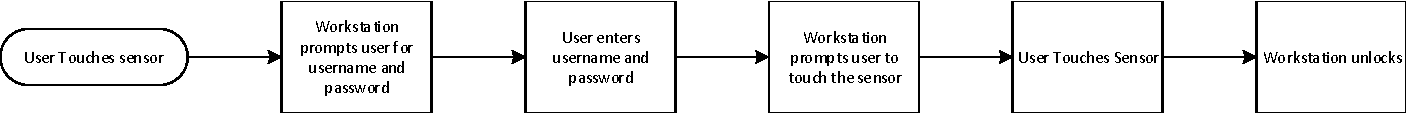
\includegraphics[width=0.7\linewidth]{./UnauthenticatedUC}
%\caption[Un-Authenticated Use Case]{Un-Authenticated Use Case}
%\label{fig:UnauthenticatedUC}
%\end{figure}

\begin{figure}[t]
\centering
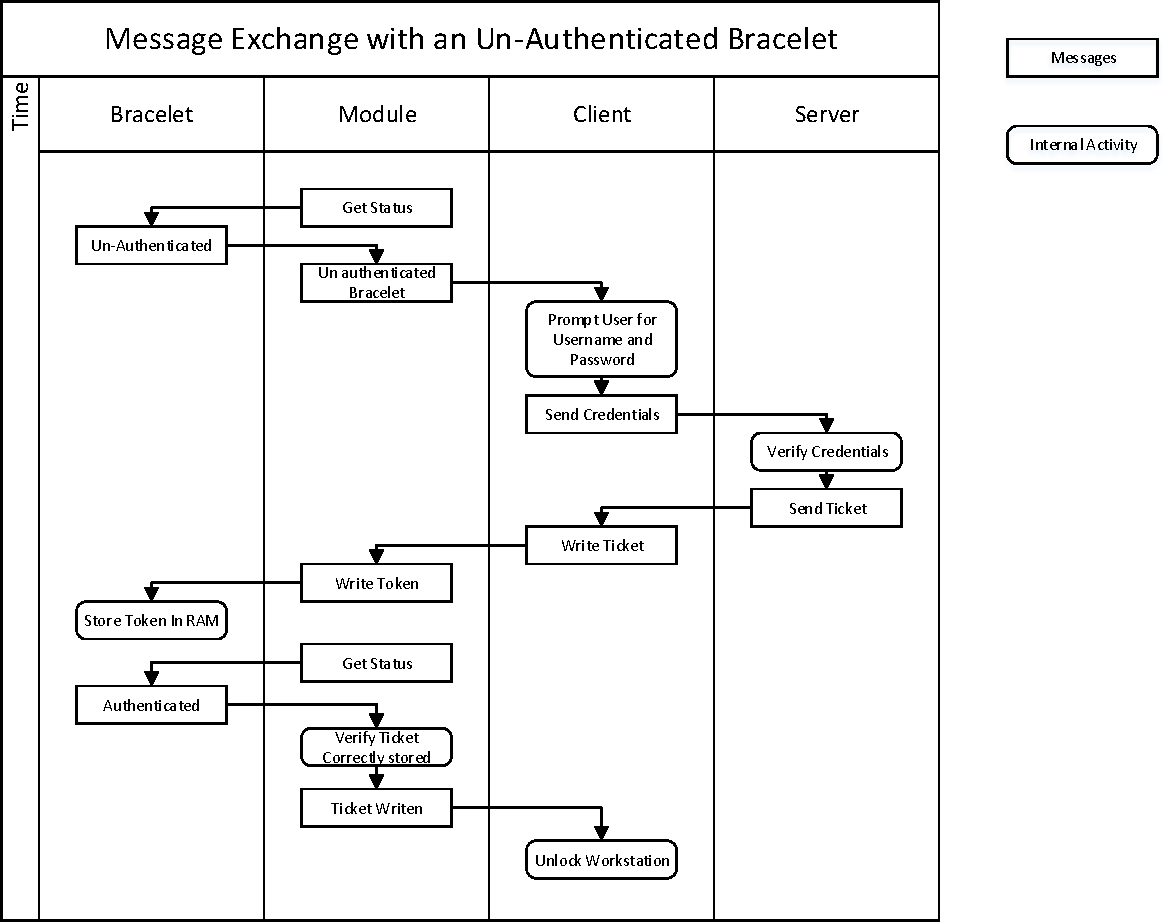
\includegraphics[width=0.7\linewidth]{./UnauthenticatedME}
\caption[Un-Authenticated Message Exchange]{Un-Authenticated Message Exchange}
\label{fig:UnauthenticatedME}
\end{figure}

%this is the original of the paragraph below
%The second use case outlines what happens when the user has a proper token stored in their bracelet.  It is described in Figure 3.  It seems very simple from the user's point of view.  The user touches the sensor on the authentication module and the workstations unlocks.  The process behind the scenes is also much simpler.  The module asks for a status, and the bracelet provides it with the token it has stored.  The module passes this information along to the clients which interoperates the token as a Kerberos ticket.  The client verifies the ticket with the Kerberos server and unlocks the workstation.  The message exchange for this use case is presented in Figure 4.

In the second use case (Figure~\ref{fig:AuthenticatedME}) the user has an authenticated bracelet.  The user touches the sensor on the authentication module.  The module asks for a status, and the bracelet provides it with the token it has stored.  The module passes this information along to the client which interprets the token as a Kerberos ticket.  The client verifies the ticket with the Kerberos server and unlocks the workstation.  Our goal is to perform this use case in less than one second.

%\begin{figure}
%\centering
%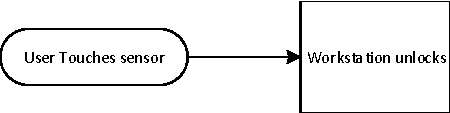
\includegraphics[width=0.25\linewidth]{./AuthenticatedUC}
%\caption[Authenticated Use Case]{Authenticated Use Case}
%\label{fig:AuthenticatedUC}
%\end{figure}

\begin{figure}[t]
\centering
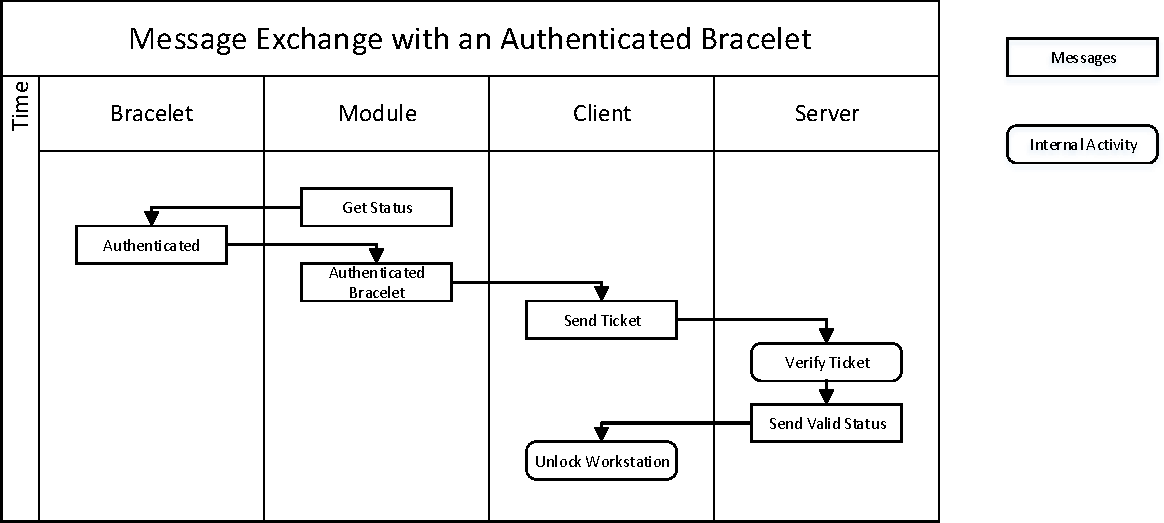
\includegraphics[width=0.7\linewidth]{./AuthenticatedME}
\caption[Authenticated Message Exchange]{Authenticated Message Exchange}
\label{fig:AuthenticatedME}
\end{figure}

%%%%%%%%%%%%%%%%%%%%%%%%%%%%%%%%%%%%%%%%%%%%%%%%%%%%%%%%%%%%%%%%%%%%%%%%%%%%%%%
\section{Experiments and Results}\label{sec:results}
%%%%%%%%%%%%%%%%%%%%%%%%%%%%%%%%%%%%%%%%%%%%%%%%%%%%%%%%%%%%%%%%%%%%%%%%%%%%%%%
\subsection{Prototype}
The hardware prototypes for the bracelet and the authentication module are based on the Atmel ATMega328 microcontroller operating at 20 MHz and an LM358AN Amplifier.  Both the bracelet and the authentication module have copper pads that make contact with the user's skin.  The signal from the skin is fed into the amplifier and the signal to the skin is driven by setting a pin on the microcontroller.  We also built a resistive analogue to represent the resistance from a user's wrist to their finger tip.  The prototype for the authentication client has been written in Python.
\subsection{Results}
Initial results are encouraging.  We are able to send commands from the authentication module to the bracelet.  The bracelet can correctly interpret those commands and it responds when issued a Get Status command.   The time elapsed for a Get Status command and a status message with a 256 byte token is approximately 500 milliseconds.  
We also implemented the functionality that clears the authentication information when the bracelet is removed.  This was accomplished by using one of the hardware interrupts on the microcontroller. 
\subsection{Hurdles}
We encountered two major hurdles during the development of the first prototype.  First, in order to successfully send a signal the bracelet and the authentication module must have a common reference for voltage.  Second, while we have been able to get the signal to transmit from the authentication module to the bracelet, we have not been able to get the signal to travel in the opposite direction and arrive in a way that the signal can be interpreted by the authentication module.  To solve both of these issues, we plan on changing the method by which the signal is transmitted over the user's skin to capacitive coupling.

%%%%%%%%%%%%%%%%%%%%%%%%%%%%%%%%%%%%%%%%%%%%%%%%%%%%%%%%%%%%%%%%%%%%%%%%%%%%%%%
\section{Future Work}\label{sec:future}
%%%%%%%%%%%%%%%%%%%%%%%%%%%%%%%%%%%%%%%%%%%%%%%%%%%%%%%%%%%%%%%%%%%%%%%%%%%%%%%
Future work will focus on improving the system.  We plan to implement the system using a microcontroller that can store larger keys.  The Atmel ATMega328 only has 2 kilobytes of ram.  Since the systems needs some ram to perform operations, the key that is stored in RAM is limited to about 1 kilobyte.  This is not sufficient space to store authentication information in real world environments.  We also plan on hardening the system by adding pre-shared message authentication codes (MACs) to protect against replay attacks.

%In the long term, we may continue the development of the system model to include a system where passwords are not required at all.  A user would check in with a security technician who would personally and physically validate the user's identity then provide the user with a bracelet and assist authenticate the user without the user entering any information into a computer.  Finally we plan on submitting the system for internal review to get it clear for testing on human subjects.


%%%%%%%%%%%%%%%%%%%%%%%%%%%%%%%%%%%%%%%%%%%%%%%%%%%%%%%%%%%%%%%%%%%%%%%%%%%%%%%
%%%%%%%%%%%%%%%%%%%%%%%%%%%%%%%%%%%%%%%%%%%%%%%%%%%%%%%%%%%%%%%%%%%%%%%%%%%%%%%
\section{References}\label{sec:references}
%%%%%%%%%%%%%%%%%%%%%%%%%%%%%%%%%%%%%%%%%%%%%%%%%%%%%%%%%%%%%%%%%%%%%%%%%%%%%%%


\bibliographystyle{splncs03}
\bibliography{paper}

%%%%%%%%%%%%%%%%%%%%%%%%%%%%%%%%%%%%%%%%%%%%%%%%%%%%%%%%%%%%%%%%%%%%%%%%%%%%%%%

\end{document}
